\documentclass{article}

\usepackage{graphicx}

\author{Dorian Arnold, Aurelien Bouteiller, George Bosilca,\\
 Kurt Feirrera, Thomas Herault, Yves Robert}
\title{Coordinated Checkpointing: Coordinating at the Platform Level}

\begin{document}

\maketitle

Consider a platform that is not well balanced to do capacity checkpointing: either because the applications are doing interfering I/O, or because the I/O is a bottleneck. Production runs can still benefit significantly from CR techniques. For example, take a platform with the following characteristics:

\begin{center}
\begin{tabular}{l|c|l}
  Number of nodes & $p$             & $10^5$ \\\hline
  Node MTBF           & $\mu_{ind}$ & 25 years\\\hline
  Node memory      & $M$             & 32GB\\\hline
  Checkpoint Ratio & $\rho$         & 33\%\\\hline
  Filesystem Bandwidth & $\beta$ & 10GB/s\\
\end{tabular}
\end{center}

The time to checkpoint a capacity run is $p\frac{M \rho}{\beta} = 29h20min$. The MTBF of the machine is $\frac{\mu_{ind}}{p} = 2h11min24s$. Thus, one cannot use the first order approximation of Daly to find the optimal checkpointing time and the waste of the machine at this capacity. Since failures hit more often than it is possible to checkpoint at this size, the waste would be very close to one, because in average the application would not progress between failures (to give an example, an execution of 40 min
followed by a checkpoint, hence 30 hours total, takes $10^{26}$ hours to complete successfully in expectation).

If the machine is used at capacity for a large amount of smaller jobs, however, each application could be protected using a CR technique. Let's consider a toy example:

\begin{center}
\begin{tabular}{lcl}
  Total number of processors & $p$ & $100,000$\\\hline
  Number of 'big' applications & $n_{b}$ & 100\\\hline
  Size of 'big' applications & $b$ & 5,000\\\hline
  Number of 'small' applications & $n_{s}$ & 5,000\\\hline
  Size of 'small' applications & $s$ & 100\\\hline
  Ratio of the machine used by 'big' applications & $\alpha = \frac{b n_{b}}{p} $ & 50\%\\
\end{tabular}
\end{center}

Then, if there was no filesystem contention/interference, and all applications could checkpoint in parallel, we could apply the Daly formulae:

\begin{eqnarray}
C(q) &=& \frac{q\rho M}{\beta}\\
\mu(q) &=& \frac{\mu_{ind}}{q}\\
Waste(q, T) &=& \frac{C(q)}{T} + \frac{1}{\mu(q)}\left(\frac{T}{2}+R(q)\right)\\
Daly(q) &=& \sqrt{2\mu(q)C(q)} = \frac{\rho M}{\beta}
\end{eqnarray}

We assume that $R(q) =C(q)$ for the recovery cost. Note that the period $Daly(q)=Daly$ is independent of
$q$, because checkpoint time is linear in $q$ while MTBF is inversely proportional to $q$.
We obtain $Waste(b, Daly(b)) = 26.1\%$, and $Waste(s, Daly(s)) = 0.5\%$, which are reasonable values that these applications can expect. From a platform perspective, we can define the waste of the platform, 

$$Waste_{plat}(T_s, T_b) = \frac{s n_{s}}{p}Waste(s, T_s) + \frac{b n_{b}}{p}Waste(b, T_b)$$

In the ideal case, $Waste_{ideal} = Waste_{plat}(Daly(s), Daly(b)) = 13.3\%$.

However, to achieve this performance, applications must checkpoint every $Daly \approx 11h20min$.
Since there are $n_b = \frac{\alpha p}{b} = 10$ 'big' applications and $n_s = \frac{(1-\alpha)p}{s} = 500$ 'small' applications, and 'big' applications take $C(b) = 1h28min$ while 'small' applications take $C(s) = 16min16s$ to checkpoint on the filesystem without interference, the time it takes to checkpoint all applications once without interference is $T_{min} = n_bC(b) + n_sC(s) = C(p) >> Daly$.

If we apply a simple round-robin strategy, allowing each application to checkpoint in turn, we obtain

$$
\begin{array}{rl}
Waste(s, T_{min}) &= 0.76\%\\
Waste(b, T_{min}) &= 38.5\%\\
\end{array}
$$

Although the small applications are not really impacted by a much larger period, big ones are impacted significantly. The platform waste using the round robin strategy in that case is $Waste_{rr} = Waste_{plat}(T_{min}, T_{min}) = 19.63\%$, 1.47 times higher than the ideal waste.

Based on this observation, one can decide to checkpoint more often the big applications: if every $n_bC(b)$ checkpoints of big applications we checkpoint only a fifth of the small applications, the period for big applications becomes $U = n_bC(b)+100C(s) = 17h36min$, and the period for small applications becomes $5(n_bC(b)+100C(s)) = 3 days 16h$, and the platform waste $Waste_{unfair} = Waste_{plat}(U, 5U) = 15\%$ (1.12 times higher than the ideal waste). Thus, hindering small applications in the case of I/O interference in favor of big ones turns out positive for the global platform efficiency in that case.

The goal of this paper is to find an efficient platform priority scheduling, when it is not possible to accommodate the optimal checkpointing period of all applications that run in parallel.

\pagebreak

\appendix
\section{Initial Thoughts}

Consider a platform with $p$ computing nodes. On this platform, at a given time job scheduler assigned $n$ applications that span on $S_{i, 1 \leq i \leq n}$ processors ($\sum_{i=1}^{n}S_i = p$). If each application uses coordinated checkpoint/restart and the same Daly formula for their checkpointing interval, is it possible to schedule all of them so that two applications never interfere?

Let $M$ be the average checkpoint size for a single node; let $b_{io}$ be the I/O bandwidth of the machine. For the sake of simplicity, consider first that there is no local I/O contention (the local link is not the bottleneck): Let $C(q)$ be the checkpoint duration of an application with $q$ nodes.

$$C(q) = q\times \frac{M}{b_{io}}$$

Let $\mu(q)$ be the MTBI of an application using $q$ nodes. By Daly, the optimal checkpoint interval of the application assuming no contention is $T_{opt}(q) = \sqrt{2C(q)\mu(q)}$. Assuming independent failures, $\mu(q) = \frac{\mu_{ind}}{q}$ (were $\mu_{ind}$ is the MTBF of a single node). Thus,

$$T_{opt}(q) = \sqrt{2\times q\times \frac{M}{b_{io}} \times \frac{\mu_{ind}}{q}} = \sqrt{2\frac{M}{b_{io}}\mu_{ind}} = T_{opt}$$

All applications checkpoint with the same interval, independent of their size (this is because the checkpoint duration is directly proportional to the number of nodes, while the chance of completing within the next time unit is inverse proportional to the same number of nodes).  To avoid contention, we thus must ensure that $\sum_{i = 1}^{n} C(S_i) \leq T_{opt}$, thus that

$$\begin{array}{rl}
\sum_{i = 1}^{n} S_i\times \frac{M}{b_{io}} & \leq \sqrt{2\frac{M}{b_{io}}\mu_{ind}}\\
p\frac{M}{b_{io}} & \leq \sqrt{2\frac{M}{b_{io}}\mu_{ind}}\\
b_{io} & \geq \frac{M\times p^2}{2\mu_{ind}}
\end{array}$$

\begin{figure}[h!]
  \begin{center}
    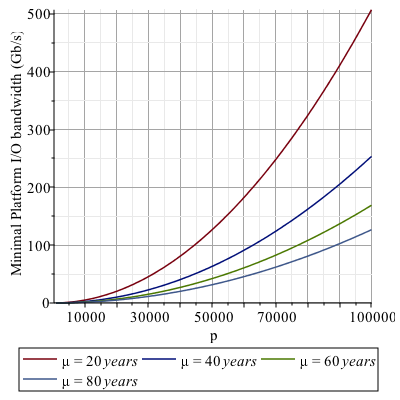
\includegraphics[width=.6\linewidth]{biomin.png}
  \end{center}
  \caption{Minimal platform I/O bandwidth requirement to allow independent checkpoint intervals\label{fig:minio}}
\end{figure}
 
Instantiating with $M = 8GB$, $p$ varying between 1,000 and 100,000, and $\mu_{ind}$ between 20 years and 80 years, we get Figure~\ref{fig:minio}. So... There is no problem? Indeed, if the platform can checkpoint a capacity application at the Daly optimal period, there is no problem. Projected machines seem to be able to do so for reasonable $\mu_{ind}$. Let's illustrate this in Figures~\ref{fig:csa-fs}, \ref{fig:csa-nvram}, \ref{fig:exa}: for a few machines, with a varying $\mu_{ind}$, this figure shows the waste using Daly optimal period (when defined) assuming the checkpoints use 60\% of the memory. Machines are described below:

\begin{description}
\item[Cori] Found in Jeff Vetters slides at the scheduling workshop: Memory is 1 PB, with 1.5PB of NVRAM. 9,300 nodes, 744GB/s I/O bandwidth. As the NVRAM is large enough to store twice 60\% of the main memory, we consider two subsystems: CoriNVRAM, where the checkpoints are stored scalably on NVRAM (at 10GB/s/node), and CoriFS, where checkpoints are stored into the main filesystem (at 744GB/s/system)
\item[Summit] Found in Jeff Vetters slides at the scheduling workshop: Memory is 1.74PB, with 2.8PB of NVRAM. 3,500 nodes, 1TB/s I/O bandwidth. As for Cori, we consider SummitNVRAM and SummitFS
\item[Aurora] Found in Jeff Vetters slides at the scheduling workshop: Memory is 7 PB, with 'on package memory local memory and persistant memory.' This is unclear what it means, so for AuroraNVRAM, we take the option 2.3PB main, 4.6PB NVRAM, and for AuroraFS, we take 7PB main. 50,000 nodes, 1TB/s I/O bandwidth.
\item[exa] Found in Jeff Vetters slides at the scheduling workshop: Memory is 32PB to 64PB, 100,000 to 1,000,000 nodes, I/O bandwidth between 30TB/s and 60TB/s. We consider the 8 options: exa1 (32PB, $10^5$, 30TB/s), exa2 (64PB, $10^5$, 30TB/s), exa3 (32PB, $10^6$, 30TB/s), exa4 (64PB, $10^6$, 30TB/s), exa5 (32PB, $10^5$, 60TB/s), exa6 (64PB, $10^5$, 60TB/s), exa7 (32PB, $10^6$, 60TB/s), exa8 (64PB, $10^6$, 60TB/s)
\end{description}

\begin{figure}[h!]
\begin{center}
  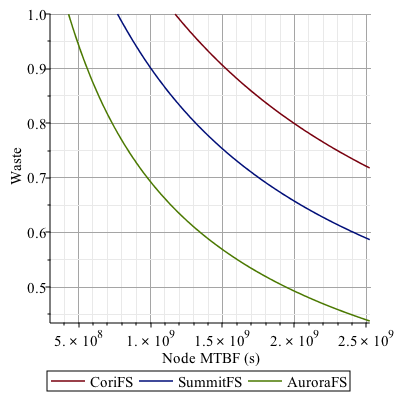
\includegraphics[width=.6\linewidth]{csa-fs.png}
\end{center}
\caption{Minimal platform checkpoint time on the filesystem for Cori, Summit and Aurora, as a ratio of the machine MTBF, and function of the MTBF of a single node (in s)\label{fig:csa-fs}}
\end{figure}

\begin{figure}[h!]
\begin{center}
  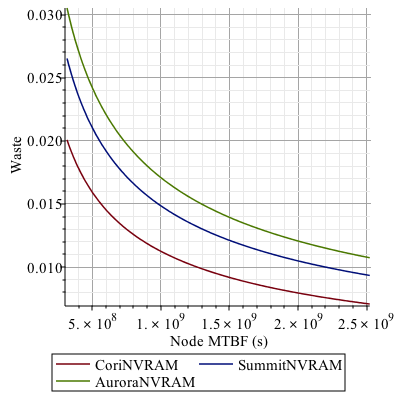
\includegraphics[width=.6\linewidth]{csa-nvram.png}
\end{center}
\caption{Minimal platform checkpoint time on their local NVRAM for Cori, Summit and Aurora, as a ratio of the machine MTBF and function of the MTBF of a single node (in s)\label{fig:csa-nvram}}
\end{figure}

\begin{figure}[h!]
\begin{center}
  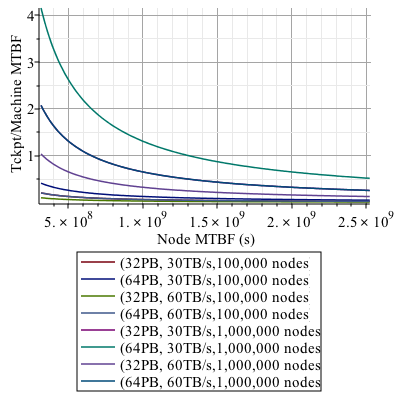
\includegraphics[width=.6\linewidth]{exa.png}
\end{center}
\caption{Minimal platform checkpoint time on the filesystem for exascale putative machines, as a ratio of the machine MTBF and function of the MTBF of a single node (in s)\label{fig:exa}}
\end{figure}

\clearpage
\section{Another model}

Consider $n$ applications on a platform with $p$ processors of individual MTBF $\mu$.
 Application $A_{i}$ has $q_{i}$ processors and checkpoint time $C_{i}$. We can
 assume that $p = \sum_{i=1}^{n} q_{i}$.
Here we do not assume that $C_{i} = q_{i} C_{\textit{base}}$ because each application could save a different total volume of data. The MTBF of $A_{i}$ is $\mu_{i} = \frac{\mu}{q_{i}}$.

We aim at building a periodic pattern of length $T$ such that each $A_{i}$ checkpoints $n_{i}$ times
within the pattern. Thus $T  = \sum_{i=1}^{n} n_{i} C_{i}$, and the $n_{i}$ (which we assume
to take rational values instead of integer ones) are the unknown. 

Application $A_{i}$ has $n_{i}$ periods of length $w_{i}+C_{i}$, where $n_{i} (w_{i}+C_{i})=T$
(we can assume equality, if we had idle time e would increase the work chunk $w_{i}$.
What is the waste? The waste for $A_{i}$ is 
$$Waste_{i} = \frac{n_{i} C_{i}}{T} + \frac{1}{\mu_{i}} (LostWork_{i} + R_{i})$$
and for the platform, $Waste = \sum_{i=1}^{n} \frac{q_{i}}{p} Waste_{i}$.


Assume $A_{i}$ can checkpoint without delay. Then $LostWork_{i} = \frac{1}{2} (w_{i}+C_{i}) = \frac{T}{2n_{i}}$.
This is  optimistic, because even though we can schedule the I/O, there is little chance that checkpoints can be equally spaced for each application.
Still, in that case we can solve and compute the $n_{i}$, at least numerically. Let $m_{i} =  \frac{n_{i} C_{i}}{T}$, we want to minimize 
$$Waste = \frac{1}{p} \sum_{i=1}^{n} q_{i} (m_{i} +  \frac{q_{i} C_{i}}{2 \mu m_{i}})$$ 
subject to $\sum_{i=1}^{n} m_{i} = 1$.

Using Lagrange multipliers, we minimize $Waste - \gamma (\sum_{i=1}^{n} m_{i} - 1)$
by zeroing out the $n$ partial derivates for each $m_{i}$ and $\gamma$ and obtain
$q_{i} - \frac{q_{i}^{2} C_{i}}{2 \mu m_{i}^{2}} - \gamma = 0$ for all $i$ (and the constraint
$\sum_{i=1}^{n} m_{i} = 1$ for $\gamma$). This leads to 
$$m_{i} = \sqrt{\frac{q_{i}^{2} C_{i}}{2 \mu (q_{i} - \gamma)}}$$
and we find $\gamma$ numerically from $\sum_{i=1}^{n} m_{i} = 1$.



\end{document}